\chapter{Git Branching}
\label{cha:git_branching}
This chapter focuses on the git commands which are responsible for creating and switching between diverging versioning timelines. The timelines can be worked on independently from each other. These diverging versioning timelines are called \dq{}branches\dq{}. After finishing this chapter, the reader is able to view all existing branches, checkout any existing branch, merge different branches and set a new beginning point for any branch.

\textit{Additional Information}: Every branch has a branch-pointer. This pointer points at the latest commit of the given branch. The main difference between the branch-pointer and the HEAD (defined in \nameref{cha:git_basics}) is that the HEAD is actually pointing at the branch-pointer of the current branch. Thus, the HEAD is only indirectly pointing at the latest commit which is dependent on the current branch, as seen in (\ref{fig:branch_pointer}).
Every git repository has a \dq{}master\dq{} branch. This branch is the main branch from which all other branches may originate.
\begin{figure}[H]
    \centering
    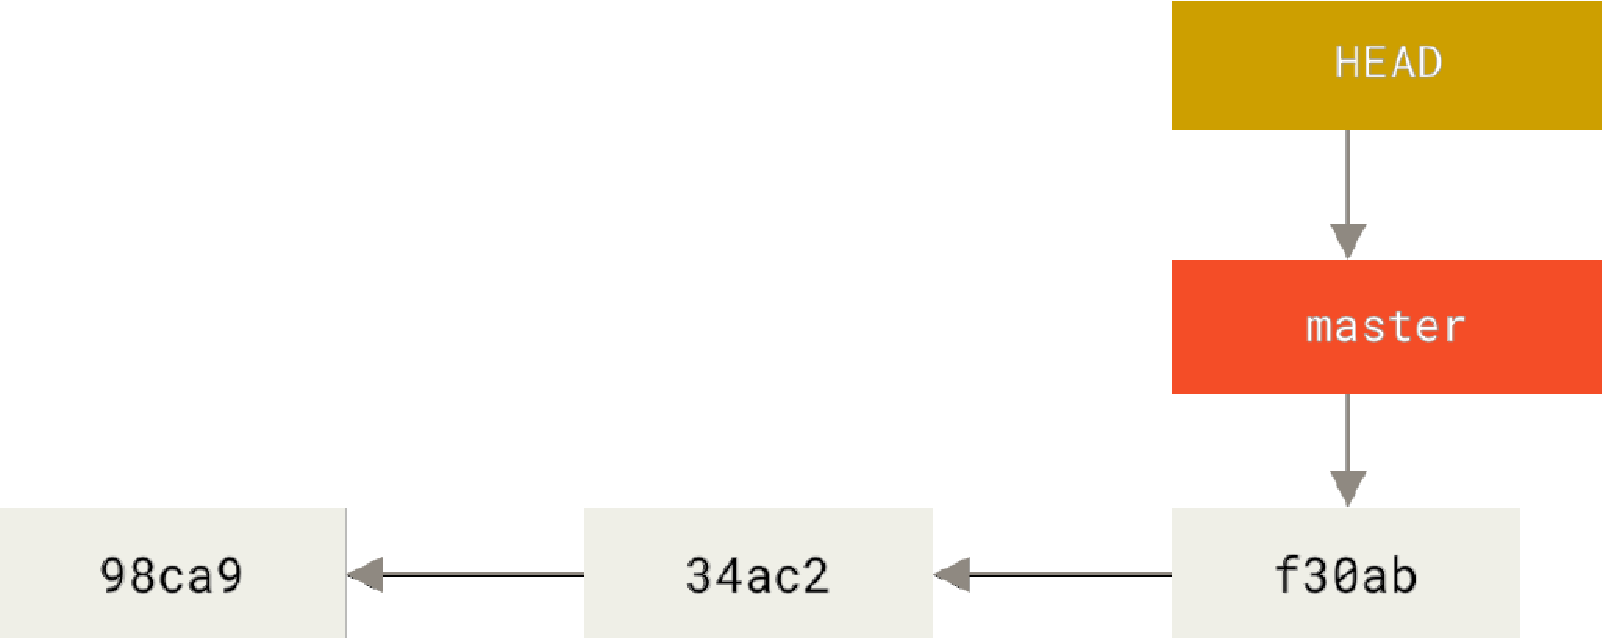
\includegraphics[width=\textwidth]{git_manual/figures/branch_pointer.pdf}
    \caption{The master branch pointer points at the latest commit. The HEAD points at the current branch which is the master \cite{CS20}.}
    \label{fig:branch_pointer}
\end{figure}

\newpage

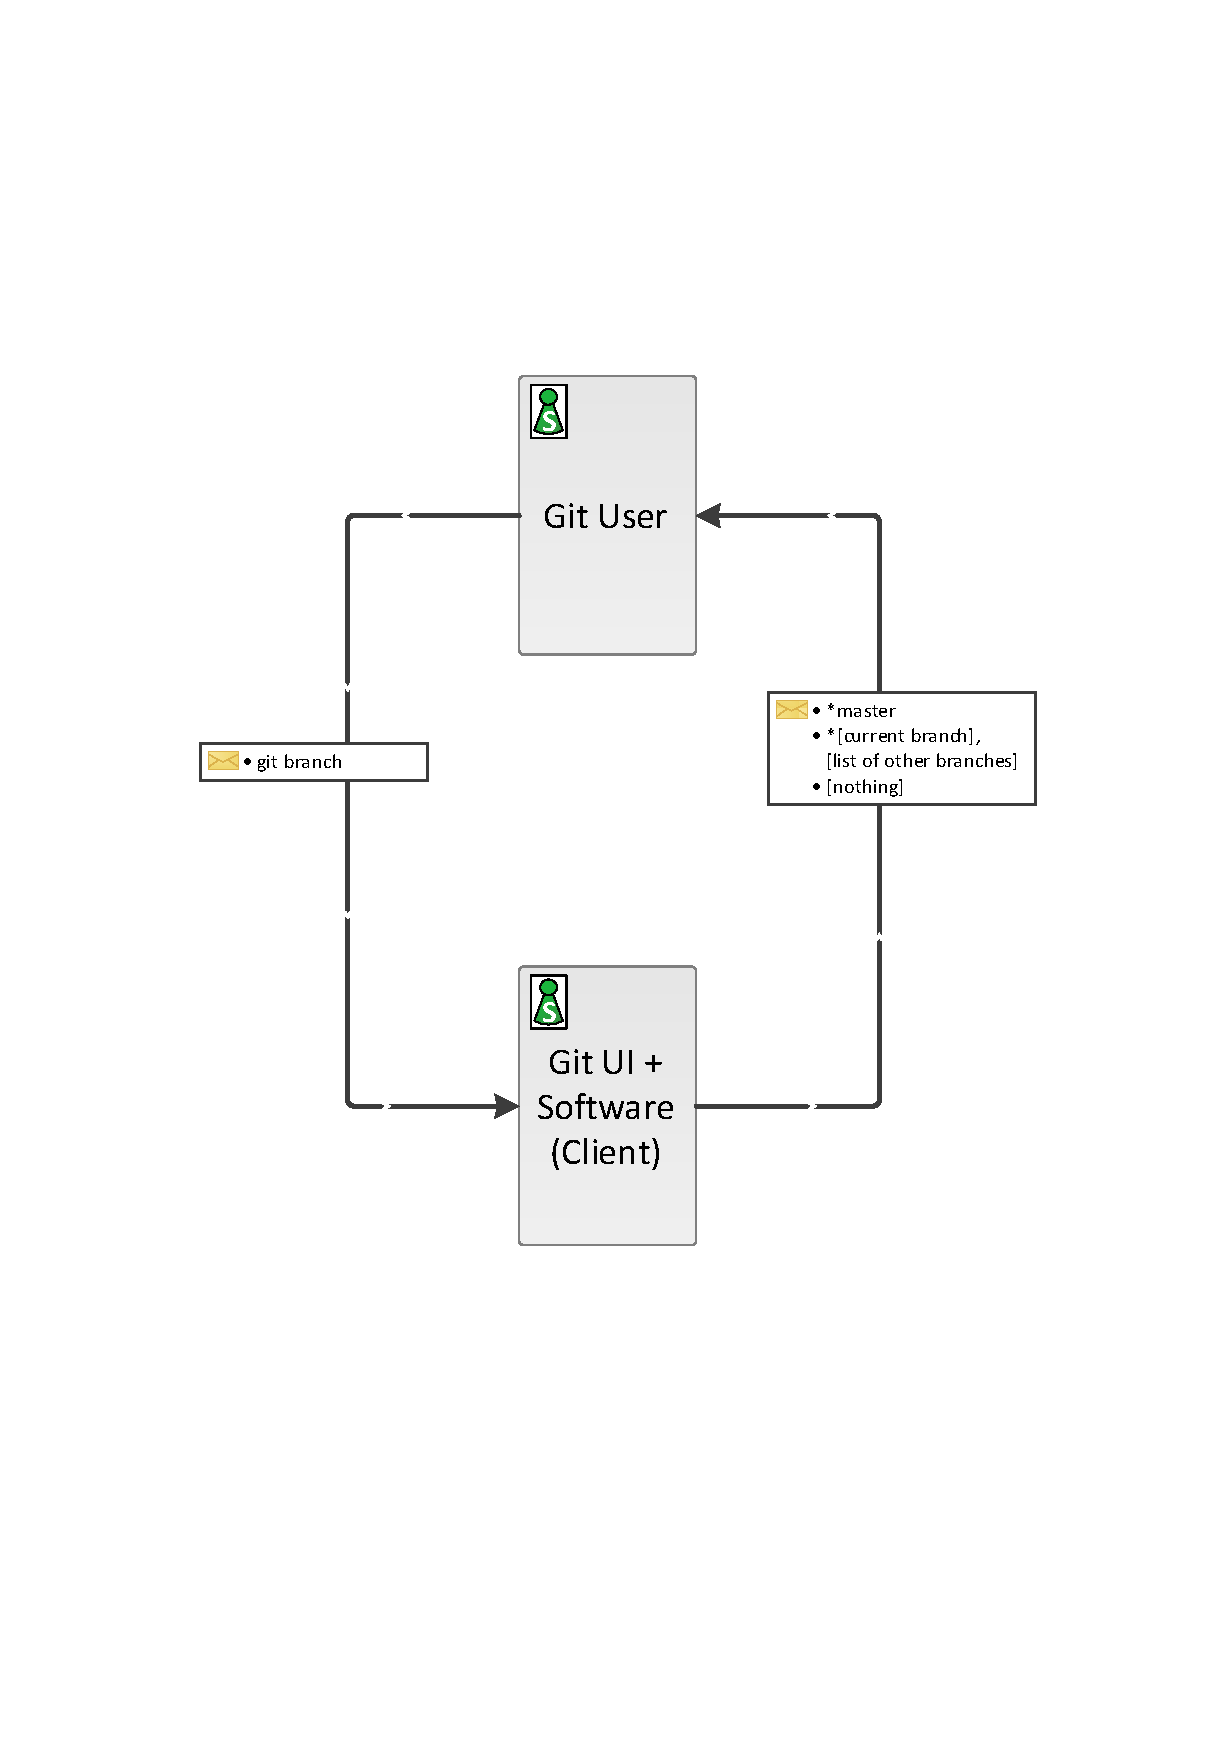
\includepdf[pages=1,pagecommand= {\section{git branch} \label{sec:git_branch} \subsection{git branch}},scale=0.9]{git_commands/git_branch.pdf}
\includepdf[pages=2-last,pagecommand={} ,scale=0.75]{git_commands/git_branch.pdf}

\newpage

\includepdf[pages=1,pagecommand= {\subsection{git branch [name]}},scale=0.9]{git_commands/git_branch_name.pdf}
\includepdf[pages=2-last,pagecommand={} ,scale=0.75]{git_commands/git_branch_name.pdf}

\newpage

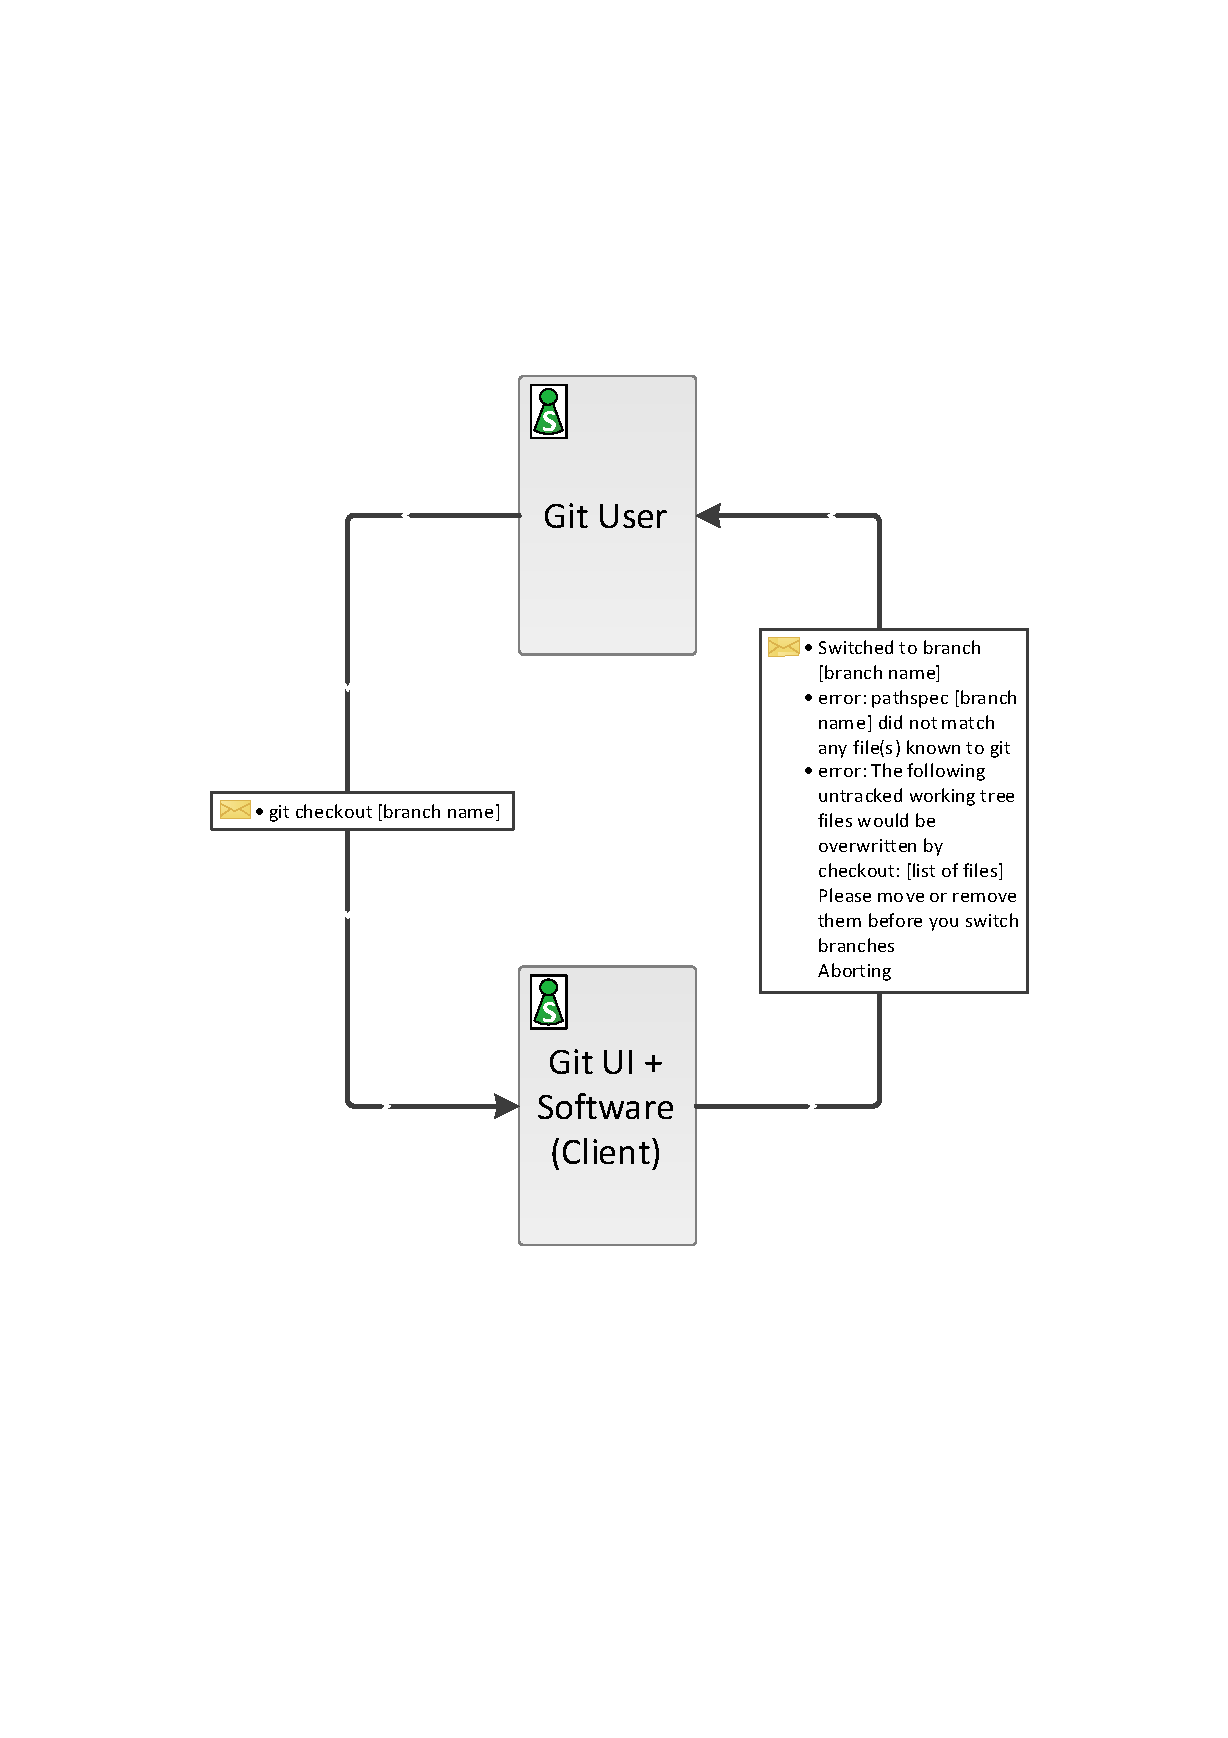
\includepdf[pages=1,pagecommand= {\section{git checkout} \label{sec:git_checkout}},scale=0.9]{git_commands/git_checkout.pdf}
\includepdf[pages=2-last,pagecommand={} ,scale=0.75]{git_commands/git_checkout.pdf}

\newpage

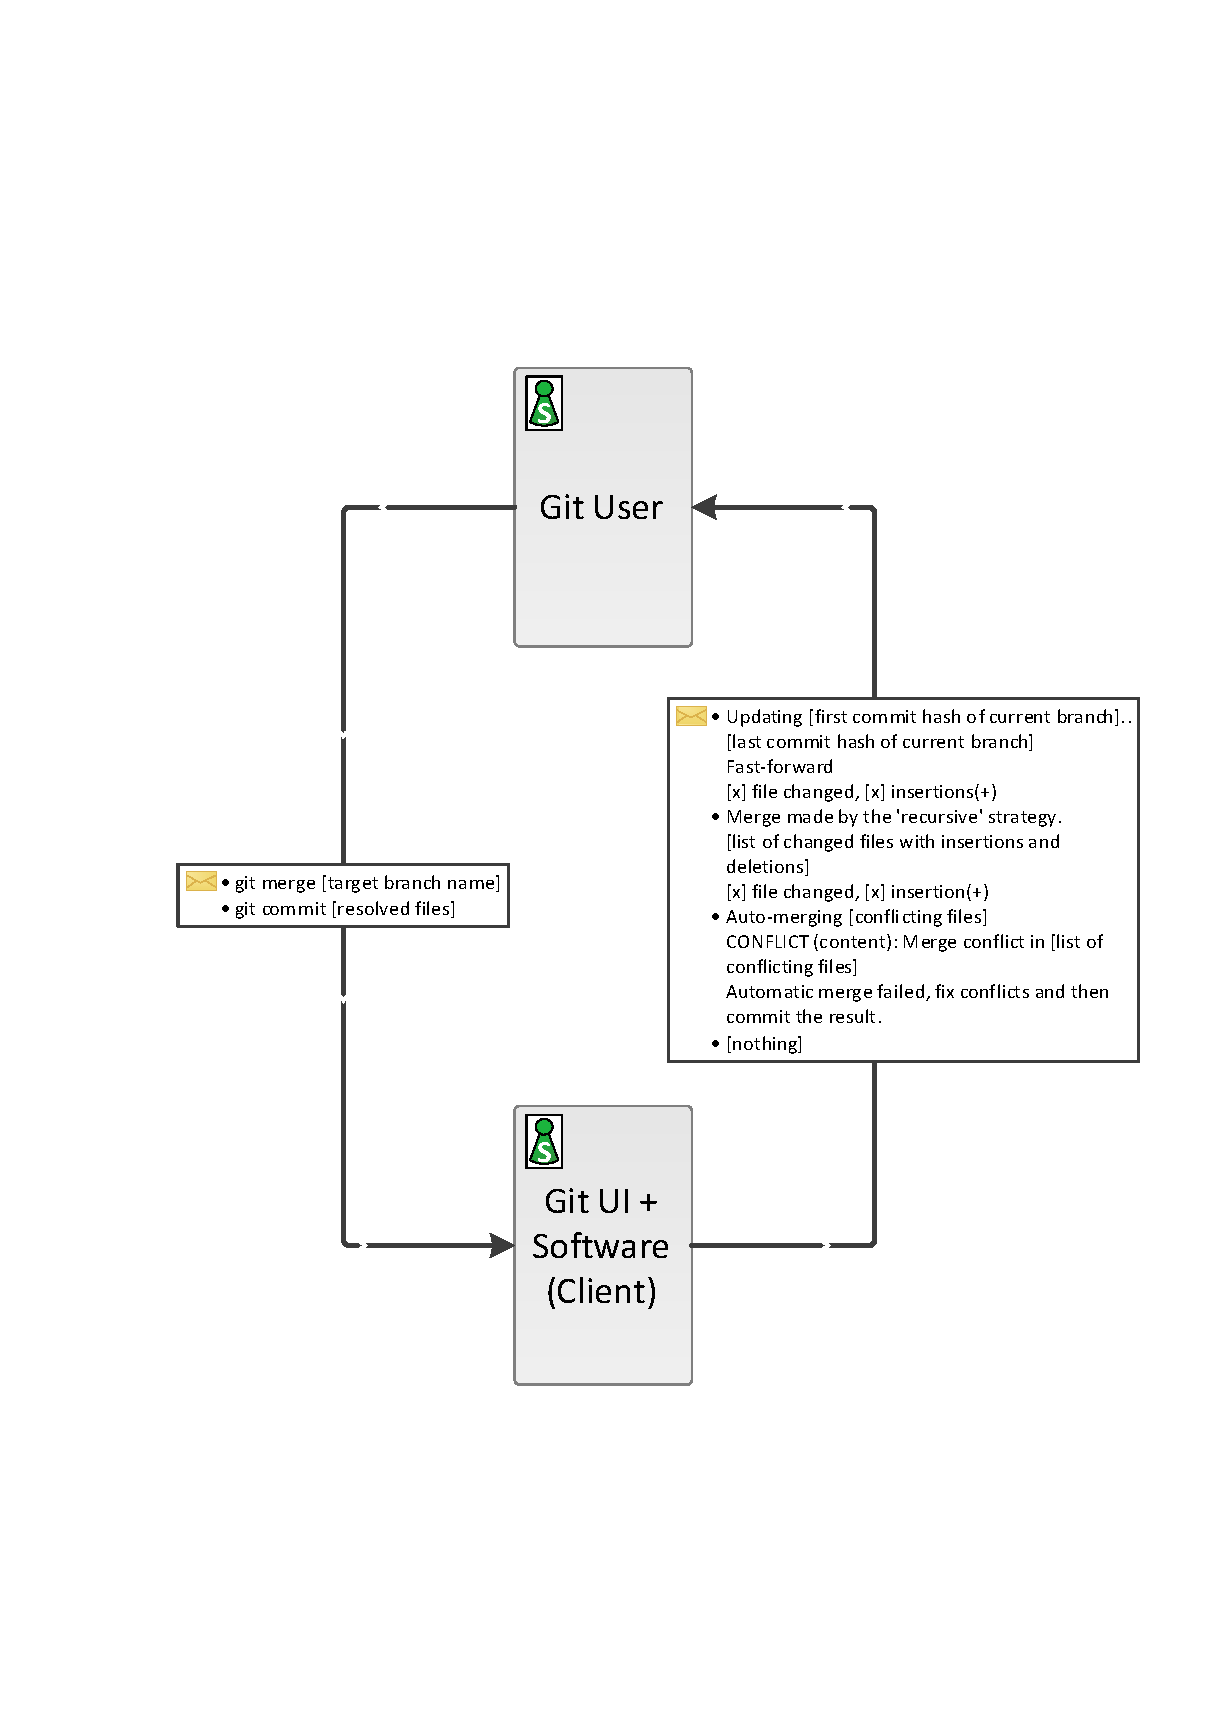
\includepdf[pages=1,pagecommand= {\section{git merge} \label{sec:git_merge}} ,scale=0.9]{git_commands/git_merge.pdf}
\includepdf[pages=2-last,pagecommand={} ,scale=0.75]{git_commands/git_merge.pdf}

\newpage

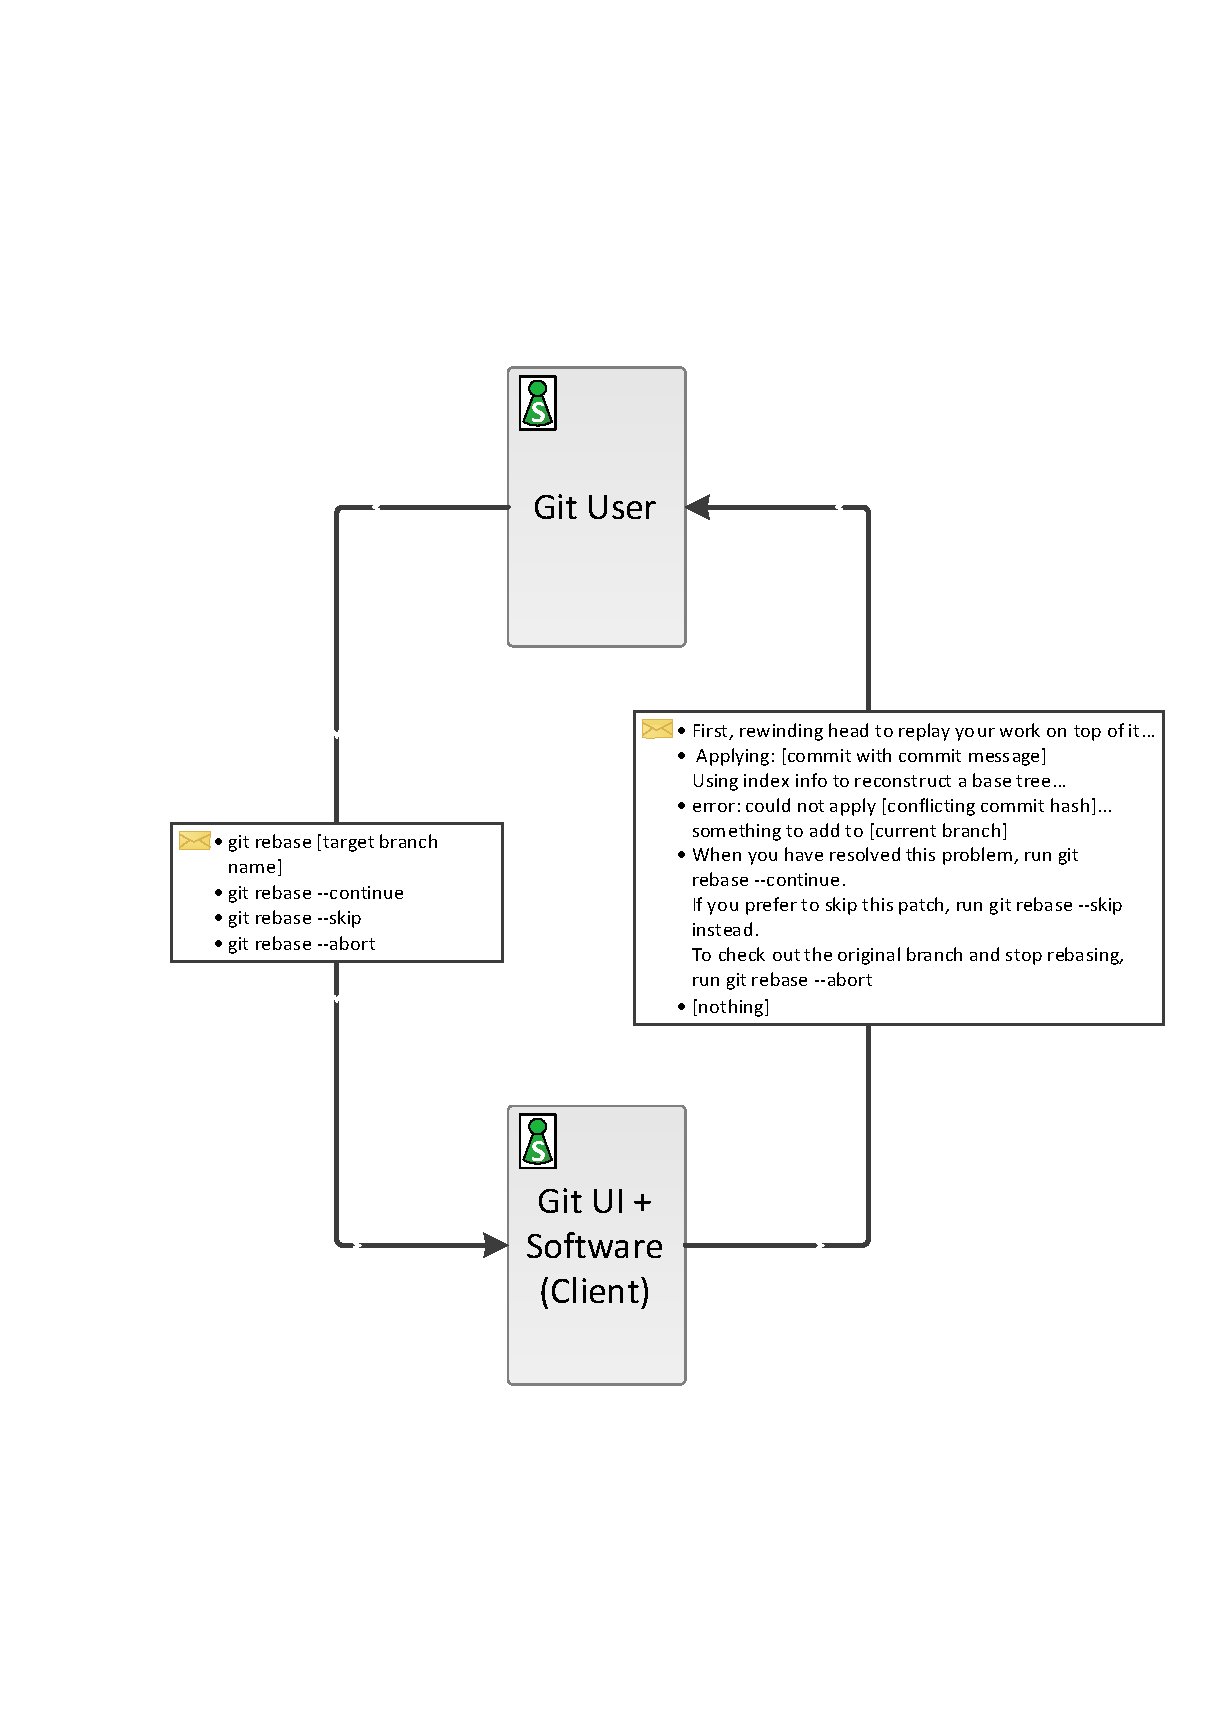
\includepdf[pages=1,pagecommand= {\section{git rebase} \label{sec:git_rebase}} ,scale=0.9]{git_commands/git_rebase.pdf}
\includepdf[pages=2,pagecommand={} ,scale=0.8]{git_commands/git_rebase.pdf}
\includepdf[pages=last,pagecommand={} ,scale=0.81]{git_commands/git_rebase.pdf}